\documentclass[11pt,twocolumn]{article}

\usepackage{epsfig}
\usepackage{graphicx}
\usepackage{graphpap}
\usepackage{amsmath}
\usepackage[utf8]{inputenc}
\usepackage[spanish]{babel}

\topmargin -2.5 cm
\textheight 9.5in
\oddsidemargin -1cm
%\evensidemargin -1cm
\textwidth 18cm
%opening
\title{}
\author{}
\date{}

\newcommand{\abre}{\textquestiondown}

\begin{document}

\pagestyle{empty}
\sffamily
\twocolumn[
Física de campos. TALLER 2: \textbf{Gravitación}

\hrulefill 
\vspace{0.3 cm}
]
\footnote{Las figuras de este documento han sido tomadas en su gran mayoría de Physics For Scientist and Engineers 6E By Serway and Jewett.}

\begin{enumerate}

\item Calcule la masa del Sol usando el hecho de que el periodo de la Tierra alrededor del Sol es $P \approx 3.156 \times 10^{7}$ s y la distancia desde el centro de la Tierra al centro del Sol es $r \approx 1.496 \times 10^{11}$ m. ¿Importa el hecho de que la Tierra y el Sol no son masas puntuales?

\item Usando el radio de la Tierra $R \approx 6.37 \times 10^{6}$ m y el hecho de que la gravedad en la superficie terrestre es $g \approx 9.8$ m$/$s$^{2}$, demuestre que la densidad promedio de la Tierra es $\rho \approx 5.51 \times 10^{3}$ $\text{kg}/\text{m}^{3}$.

\item Considere un satélite de masa $m$ en órbita circular alrededor de la Tierra, a una rapidez constante $v$ y a una altitud $h$ por encima de la superficie terrestre (ver figura).
\begin{figure}[h]
\centering
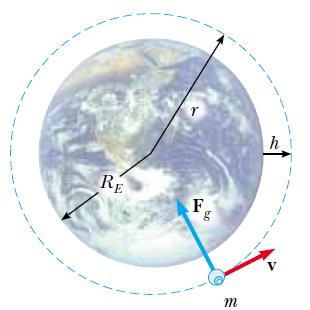
\includegraphics[scale=0.35]{fig1}
\end{figure}
\begin{enumerate}
\item Determine la rapidez del satélite en términos de $G$, $h$, $R$ (radio de la Tierra), y $M$ (masa de la Tierra).
\item ¿Cuál es la rapidez del satélite si es geoestacionario y a qué altura respecto a la superficie debe encontrarse?
\end{enumerate}

\item El cometa Halley se acerca al sol a una distancia de 0.57 A. U. (Un A. U. es igual a $1.50 \times 10^{11}$ m) y su periodo orbital es $75.6$ años. ¿Qué tan lejos del Sol viajar el cometa antes de alcanzar su jornada de regreso?
\begin{figure}[h]
\centering
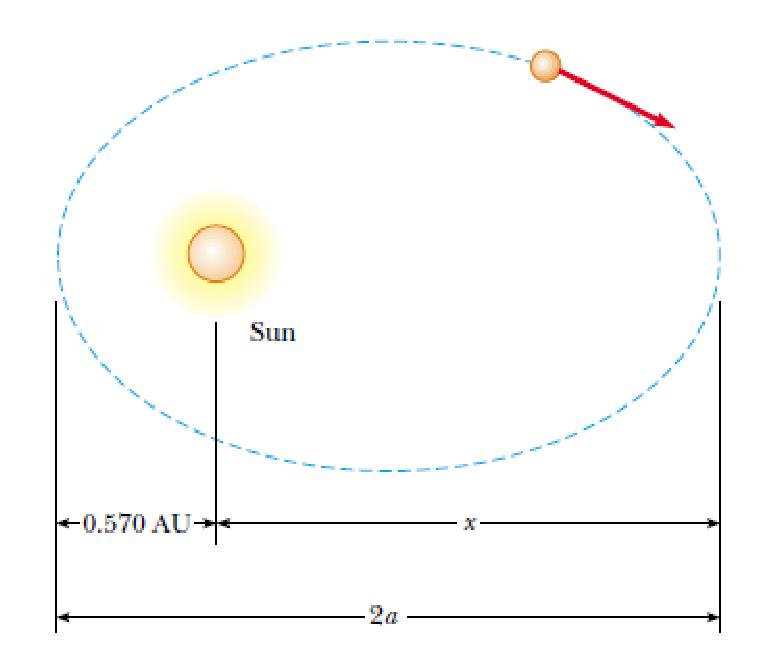
\includegraphics[scale=0.55]{fig2}
\end{figure}

\item Se ha propuesto un lugar para vivir en el espacio en forma de cilindro de $6$ km de diámetro y $30$ km de longitud (G.K. O'Neill, 1974). En dicho lugar se construirían ciudades, tierras y lagos en la superficie, con aire y nubes en el centro. Todo esto se mantendría en su lugar por la rotación del cilindro respecto a su eje mayor. ¿Qué tan rápido tendría que girar el cilindro para producir un campo gravitacional de $1 g$ (9.8 m$/$s$^{2}$) en las paredes del cilindro?


\item Calcule la magnitud y dirección del campo gravitacional en un punto P sobre el bisector de la linea que une los dos planetas de igual masa mostrados en la figura. Los planetas están separados una distancia $2a$.
\begin{figure}[h]
\centering
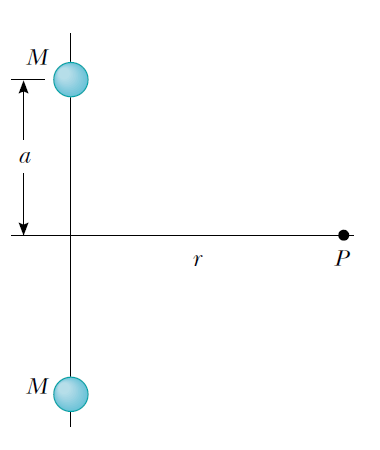
\includegraphics[scale=0.4]{fig6}
\end{figure}

\item Tres masas puntuales $m$ están localizadas en las esquinas de un cuadrado de lado $l$ (ver figura). 
\begin{enumerate}
\item Halle el campo gravitacional en el punto de coordenadas (0,0).
\begin{align*}
\vec{g}&=\dfrac{Gm}{l^2}\left(1+\dfrac{\sqrt{2}}{4}\right)\left(\hat{i}+\hat{j}\right)
\end{align*}
\item Halle la fuerza gravitacional sobre una masa $M$ que se localiza en el punto de coordenadas (0,0).
\begin{align*}
\vec{F}&= M\vec{g}=\dfrac{GMm}{l^2}\left(1+\dfrac{\sqrt{2}}{4}\right)\left(\hat{i}+\hat{j}\right)
\end{align*}
\end{enumerate}

\begin{figure}[h]
\centering
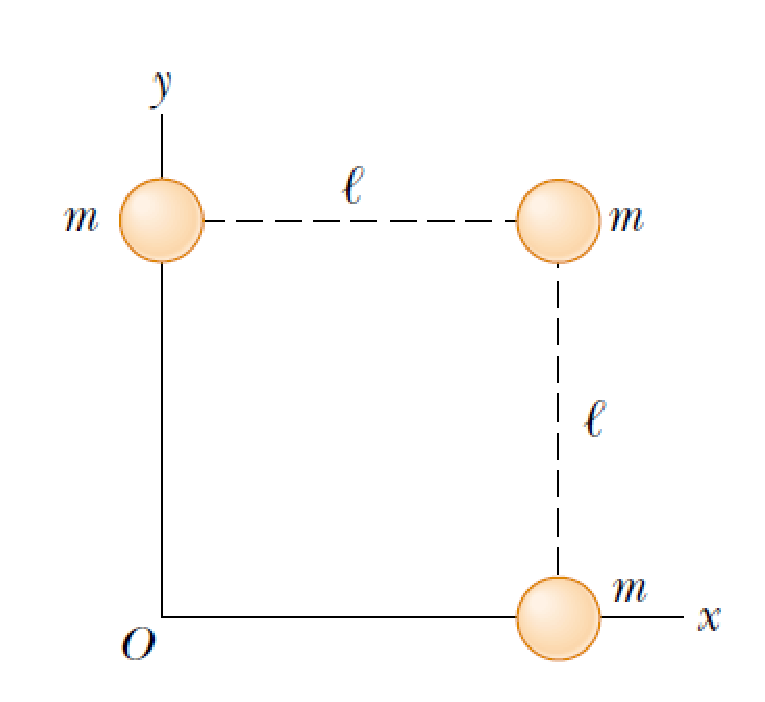
\includegraphics[scale=0.5]{fig5}
\end{figure}


%ejercicio
\item Tres masas puntuales $m$ iguales se encuentran fijas en los puntos coordenados (0,0,0), (0,0,a), (0,0,-a). Una cuarta masa $M$ describe una órbita circular de radio $R$ en un plano perpendicular al plano que contiene las tres masas anteriores y con centro en el punto (0,0,0).
\begin{enumerate}
\item Halle la magnitud de la fuerza resultante sobre la masa $M$.
\begin{align*}
F&=GMm\left(\dfrac{1}{R^2}+\dfrac{2R}{(a^2+R^2)^{3/2}}\right)
\end{align*}
\item Halle el periodo de revolución de la masa que efectúa el movimiento circular.
\begin{align*}
P&=\sqrt{\dfrac{4\pi^2R}{G m\left(\dfrac{1}{R^2}+\dfrac{2R}{(a^2+R^2)^{3/2}}\right)}}
\end{align*}
\item Encuentre la energía potencial asociada con estas cuatro masas puntuales.
\begin{align*}
U&=-Gm\left[\dfrac{5m}{2a}+M\left(\dfrac{1}{R}+\dfrac{2}{\sqrt{a^2+R^2}}\right)\right]
\end{align*}
\end{enumerate}




%ejercicio
\item El sistema binario Plaskett consiste de dos estrellas de masa iguales girando en torno a su centro de masa CM. Asuma que la rapidez de cada estrella es $v=220$ km$/$s y que el periodo orbital de cada estrella es de $14.4$ días. Halle la masa $M$ de cada estrella.
\begin{figure}[h]
\centering
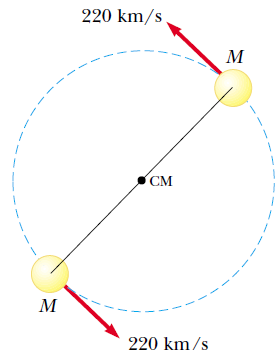
\includegraphics[scale=0.5]{fig3}
\end{figure}


%ejercicio
\item Dos estrellas de masas $m$ y $M$ , separadas por una distancia $d$, giran en órbita circular alrededor de su centro de masa CM (ver figura). Muestre que el periodo de cada estrella está dado por:
\begin{displaymath}
T^{2}=\dfrac{4\pi^{2}d^{3}}{G(M+m)}
\end{displaymath}
\begin{figure}[h]
\centering
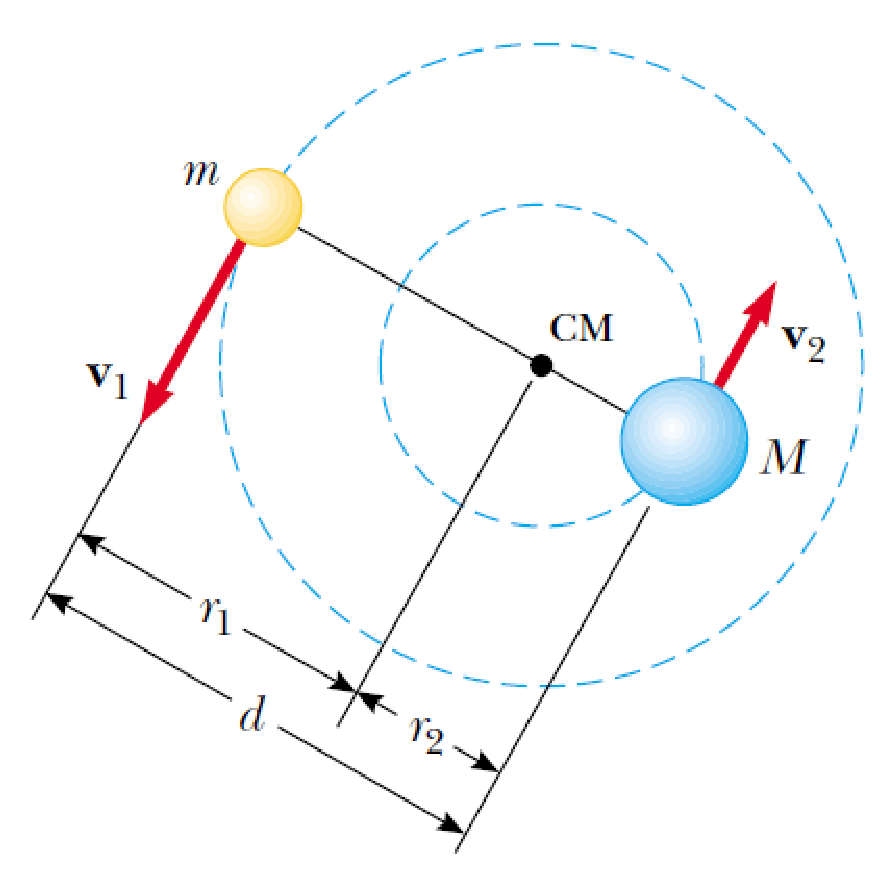
\includegraphics[scale=0.5]{fig4}
\end{figure}


%ejercicio 11
\item Un planeta hipotético de masa $M$ tiene tres lunas de igual masa $m$, cada una moviéndose en una órbita circular de radio $R$. Las lunas están igualmente espaciadas, por lo que forman un triángulo equilátero. Encuentre:
\begin{enumerate}
\item La energía potencial total del sistema.
\begin{align*}
U&=-\dfrac{3Gm}{R}\left(M+\dfrac{m}{\sqrt{3}}\right)
\end{align*}
\item La rapidez orbital de cada luna para que pueda mantenerse en esa configuración.
\begin{align*}
v&=\sqrt{\dfrac{G}{R}\left(M+\dfrac{m}{\sqrt{3}}\right)}
\end{align*}
\end{enumerate}



%ejercicio
\item Una partícula de masa $m$ se haya en un eje de simetría de un anillo de radio $R$ y masa $M$ uniformemente distribuida.
\begin{enumerate}
\item Encuentre la fuerza sobre $m$ si está a una distancia $d$ del plano del anillo.
\item Demuestre que su resultado del inciso anterior se reduce a lo que se espera intuitivamente cuando:
\begin{itemize}
\item $m$ está en el centro del anillo.
\item $m$ se encuentra distante del anillo ($d$ $>>$ $R$). 
\end{itemize}
\end{enumerate}


\item Muestre que el momento angular $L$, la excentricidad  y la energía $E$ en el movimiento general bajo interacción gravitacional, son tal que:
\begin{align*}
L^2=&GMm^2a(1-\epsilon^2)\\
\epsilon^2=&1+\dfrac{2E}{m}\left(\dfrac{L}{GmM}\right)^2\\
E=&-\dfrac{GMm}{2a}
\end{align*}

\item Muestre la tercera ley de Kepler para $M\gg m$
\begin{align*}
P^2=\dfrac{4\pi^2}{GM}a^3
\end{align*}

\item Un satélite de masa $m = 2000$ kg está en órbita elíptica alrededor de la tierra. 
En el perigeo tiene una altura de $1100$ km y el apogeo su altitud es de $4100$ km (el radio de la tierra es $R\approx 6400$ km). Determine la energía del sistema, la excentricidad  de la  orbital, el momento angular del satélite y su rapidez en perigeo y en el apogeo.

Respuesta:
\begin{align*}
E&\approx-4.5\times 10^{10}\,\text{J},\hspace{0.3 cm} \epsilon=\dfrac{1}{6}\,\\
L&=1.2\times 10^{14} \text{kg m$^2/$s}\\
v_p&\approx7900\, \text{m/s},\;\hspace{0.3 cm} v_a\approx5600\, \text{m/s}.
\end{align*}

\item Un proyectil de masa m es lanzado desde la superficie de la tierra formando un  ángulo $\alpha$ con la vertical. Si la rapidez inicial del proyectil es $v_0=\sqrt{\dfrac{GM}{R_e}}$, donde $M$ es la masa de la tierra. Determinar la altura máxima alcanzada por el proyectil ($r_{\text{max}}$).

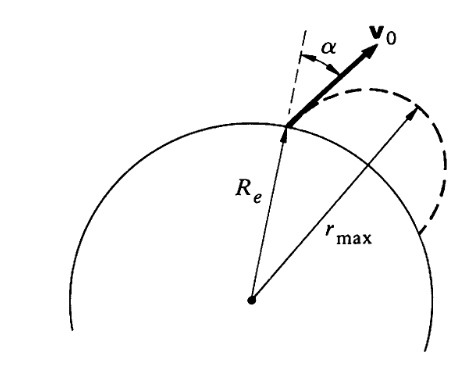
\includegraphics[scale=0.3]{tiro}
\begin{align*}
\text{Respuesta:}\hspace{0.5 cm} r_{\text{max}}=R(1+\cos\alpha)
\end{align*}

\item Un satélite de masa $m$ está en órbita circular alrededor de la tierra de masa $M$ y radio $R$ a una altura $h=R$. En un punto de la órbita hay un fallo en el motor y la rapidez disminuye instatáneamente a la mitad y después se apaga, haciendo que el satélite quede en caida libre y en una nueva órbita elíptica hasta caer a la tierra.
\begin{enumerate}
\item Hallar la magnitud de la velocidad cuando el satélite impacta sobre la tierra.
\item Hallar el semieje mayor de la órbita ($a=(8/7)R$).
\item Hallar la excentricidad de la órbita ($\epsilon=3/4$).
\end{enumerate}

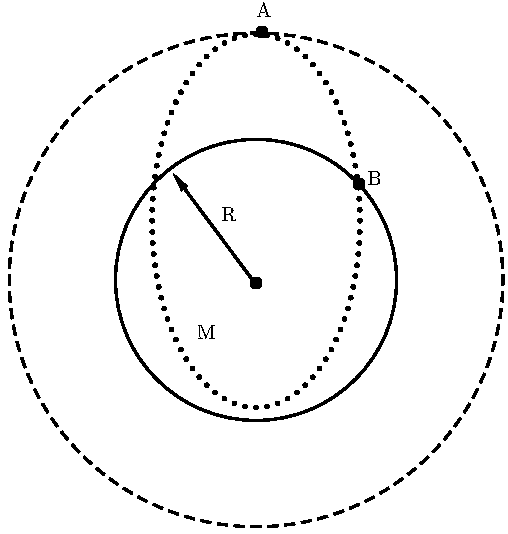
\includegraphics[scale=0.5]{orbita-choque}

\item Haga todos los cálculos de distribuciones continuas hechos y propuestos en clase.


\end{enumerate}
\end{document}
